\section{Discussion}
\label{sec:discussion}

\paragraph{\textbf{Societal Impact.}}
\framework{} aims to improve knowledge-grounded reasoning by enabling language models to interact with structured knowledge graphs through learned retrieval policies. This may benefit applications requiring factual consistency and traceable reasoning, such as question answering, scientific knowledge access, and enterprise knowledge systems. By reducing reliance on complex multi-module pipelines, \framework{} may also improve the accessibility and deployment efficiency of knowledge-grounded reasoning systems.

\paragraph{\textbf{Potential Negative Impact.}}
Like other retrieval-augmented systems, \framework{} may propagate incorrect or outdated knowledge if the underlying knowledge graph is incomplete, noisy, or maliciously manipulated. In high-stakes domains such as medicine or finance, such errors could lead to misleading outputs. Additionally, improved knowledge-grounded reasoning may be misused to automate large-scale misinformation generation with higher factual coherence.

\paragraph{\textbf{Limitations.}}
\framework{} assumes access to a reasonably structured and queryable knowledge graph, which may not be available in all domains. Its performance depends on the quality and schema consistency of the KG, and transferability may degrade under severe schema mismatch or noisy graph structures. Furthermore, while \framework{} improves inference efficiency through structured interaction, reinforcement learning training remains computationally expensive compared to standard supervised fine-tuning.

\section{Completeness and Transferability of the KG-Server}
\label{appendix:theoretical_proof}
\label{app:kg-r1-proofs}

Here, we discuss the completeness and transferability of $\mathcal{U}_{ret}$ in our KG retrieval server.

\paragraph{Preliminaries.}
Let \(G=\{(e,r,e')\mid e,e'\!\in\!\mathcal{E},\,r\!\in\!\mathcal{R}\}\) be a directed KG.
Define the \textsc{KG-R1} action set
\[
\ActSet = 
\left\{
\begin{aligned}
&\gettailrelations,\ \getheadrelations,\\
&\gettailentities,\ \getheadentities
\end{aligned}
\right\}
\]

with the following semantics for any \((e,r,e')\in G\):
\begin{align*}
\gettailrelations(e)
&:= \{\, r \in \mathcal{R} \mid \exists e'\in\mathcal{E}:\ (e,r,e')\in G \,\},\\[2pt]
\getheadrelations(e')
&:= \{\, r \in \mathcal{R} \mid \exists e\in\mathcal{E}:\ (e,r,e')\in G \,\},\\[2pt]
\gettailentities(e,r)
&:= \{\, e' \in \mathcal{E} \mid (e,r,e')\in G \,\},\\[2pt]
\getheadentities(r,e')
&:= \{\, e \in \mathcal{E} \mid (e,r,e')\in G \,\}.
\end{align*}
A \emph{relation path} is \(z=(r_1,\ldots,r_\ell)\), and a \emph{reasoning path} (instantiation) is
\[
Z:\ e_0 \xrightarrow{r_1} e_1 \xrightarrow{r_2} \cdots \xrightarrow{r_\ell} e_\ell,
\quad (e_{i-1},r_i,e_i)\in G.
\]




\completeness*


\noindent \emph{Proof.}
Starting with \(\ell=1\), if \((e_0,r_1,e_1)\in G\) then \(e_1\in\gettailentities(e_0,r_1)\).
For the inductive step, assume the claim holds for length \(\ell-1\).
By the induction hypothesis, we reach \(e_{\ell-1}\); applying \(\gettailentities(e_{\ell-1},r_\ell)\) then returns a set containing \(e_\ell\).

\vspace{1.0\baselineskip} 







\paragraph{Schema-Free Transferability.}
The retrieval action interface $\ActSet$ is defined purely in terms of set operations over triples $(e,r,e')$, independent of any schema, ontology, or datatype constraints. As a result, the same action interface can be applied to different knowledge graphs without modification. This allows a learned policy to be executed on a new KG by simply replacing the backend graph.

However, this property guarantees only that the policy remains well-defined under KG replacement. The effectiveness of transfer depends on the similarity between the training and target KGs and is evaluated empirically in Section~\ref{sec:exp2}.


\section{Datasets}
\label{appendix:datasets}

\subsection{KGQA Datasets}
Here, we list the KGQA datasets used in this paper.

\paragraph{Freebase-based Datasets}

\begin{itemize}[topsep=1pt,itemsep=2pt,parsep=0pt,leftmargin=10pt]
\item \textbf{WebQSP}~\citep{Yih2016WebQSP} (1,639 test QA pairs)
Open-domain questions with mostly 1--2 hop reasoning over Freebase MIDs and SPARQL annotations.

\item \textbf{ComplexWebQuestions (CWQ)}~\citep{Talmor2018CWQ} (3,531 test QA pairs)
Compositional multi-hop questions generated from SPARQL templates that stress longer chains and constraint composition are used to probe multi-turn retrieval quality and robustness without dataset-specific rules.

\item \textbf{SimpleQuestions (SimpleQA)}~\citep{bordes2015simplequestions} (1,000 sampled test QA pairs)
Single-relation 1-hop questions over Freebase serve as a retrieval-fidelity and token-efficiency baseline for \framework{}. We randomly sample 1{,}000 QA from the original test split (21{,}687).

\item \textbf{GrailQA}~\citep{gu2021grailqa} (1,000 sampled test QA pairs)
Diverse compositional questions emphasizing generalization under Freebase; handled with the same minimal action interface and no hand-crafted schemas. We randomly sample 1{,}000 from the original test split (13{,}231).
\end{itemize}

\paragraph{Wikidata-based Datasets}

\begin{itemize}[topsep=1pt,itemsep=2pt,parsep=0pt,leftmargin=10pt]
\item \textbf{T-REx}~\citep{elsahar2018trex} (5,000 test QA pairs)
Large-scale slot-filling–style QA grounded in Wikidata triples; used to assess scalability and coverage under a different KG schema. We randomly sample 5{,}000 from the corpus (\(\sim\)2.2M).

\item \textbf{QALD-10en}~\citep{usbeck2023qald10} (333 test QA pairs)
Manually curated, linguistically varied questions over Wikidata; useful for evaluating precision on a small but challenging set. We evaluate on 333 examples.
\end{itemize}




\subsection{Dataset Pre-processing}

\paragraph{Two-hop Subgraph Extraction Methodology.}
Following the subgraph pre-processing practice RoG~\citep{Luo2024RoG}, we build a question-specific near subgraph to shrink the search space and suppress spurious matches: starting from the linked anchor entities \(e_q\) and gold answers \(A_q\), it performs a breadth-first expansion over the KG \(G\) up to the dataset’s maximum 2-hop radius \(h\). The processed subgraph for each question is cached and used for the KG retrieval server in \framework{}.

\subsection{Freebase and Wikidata Schema Comparison}

The following tables show the different schemas of Freebase and Wikidata.
\label{tab:datasets}
\begin{longtable}{p{2cm}|p{4cm}|p{6cm}} 
\caption{Freebase knowledge graph dataset used for KGQA evaluation. All datasets share the same underlying Freebase knowledge graph structure with 4.9M entities and 663 relations.} 
\label{tab:freebase_kg_datasets} \\ 
\toprule 
\textbf{Dataset} & \textbf{Entities} & \textbf{Relations} \\ 
\midrule 
\textbf{Freebase} & 
\begin{minipage}[t]{5.2cm}
{\footnotesize 
- P!nk \\
- Gender \\
- Ice Cube \\
- United States of America \\
- Nemanja Mikic}
\end{minipage} & 
\begin{minipage}[t]{7cm}
{\footnotesize 
- broadcast.content.artist \\
- people.person.nationality \\
- music.artist\_genre\\
- location.location.containedby \\
- basketball.basketball.player\_position}
\end{minipage} \\ 
\midrule
\multicolumn{3}{l}{\textbf{Questions}} \\
\multicolumn{3}{p{12cm}}{\footnotesize 
\begin{tabular}[t]{@{}p{13.5cm}@{}}
\textbf{WebQSP (1,639 test questions):} \\
Q: What does jamaican people speak? \\
A: \textit{[Jamaican English, Jamaican Creole English Language]} \\[0.2em]
\textbf{CWQ (3,531 test questions):} \\
Q: Lou Seal is the mascot for the team that last won the World Series when? \\
A: \textit{[2014 World Series]} \\[0.2em]
\textbf{SimpleQA (21,687 test questions):} \\
Q: Where is the madam satan located? \\
A: \textit{[United States of America]} \\[0.2em]
\textbf{GrailQA (13,231 test questions):} \\
Q: Which play is produced by the illusion? \\
A: \textit{[The Illusion]}
\end{tabular}} \\ 
\bottomrule 
\end{longtable}

\begin{longtable}{p{2cm}|p{4cm}|p{6cm}} 
\caption{Wikidata knowledge graph datasets used for KGQA evaluation. All datasets share the same underlying Wikidata knowledge graph structure with 15M entities and 2.3K relations.} 
\label{tab:wikidata_kg_datasets} \\ 
\toprule 
\textbf{Dataset} & \textbf{Entities} & \textbf{Relations} \\ 
\midrule 
\textbf{Wikidata} & 
\begin{minipage}[t]{5.2cm}
{\footnotesize 
- Barack Obama \\
- Germany \\
- Albert Einstein \\
- Microsoft \\
- Paris}
\end{minipage} & 
\begin{minipage}[t]{7cm}
{\footnotesize 
- instance of \\
- country \\
- occupation \\
- date of birth \\
- place of birth}
\end{minipage} \\ 
\midrule
\multicolumn{3}{l}{\textbf{Questions}} \\
\multicolumn{3}{p{12cm}}{\footnotesize 
\begin{tabular}[t]{@{}p{13.5cm}@{}}
\textbf{T-Rex (2.2M test questions):} \\
Q: What is the occupation of Albert Einstein? \\
A: \textit{[Physicist]} \\[0.2em]

\textbf{QALD-10en (250 test questions):} \\
Q: Which companies were founded by Bill Gates? \\
A: \textit{[Microsoft]} \\[0.2em]
\end{tabular}} \\ 
\bottomrule 
\end{longtable}













\section{Baselines}
\label{appendix:baselines}


\subsection{LLM-only Methods}
\textbf{Setup.} We evaluate IO, CoT, and SC in a zero-shot setting without access to the KG retrieval server (i.e., no KG augmentation). All baselines run on Qwen2.5-7B-it, Qwen2.5-72B-it, Qwen3-235B-A22B-Instruct-2507 with temperature=0 and top\_p=50.

\noindent\textbf{Prompts.}
We use the following prompt templates for IO and CoT baselines (the SC baseline performs majority voting over CoT results and hence uses the same prompt as CoT).
\begin{tcolorbox}[colback=white, colframe=black, title=Prompte template for IO Prompt setup, boxrule=0.5pt, left=2mm, right=2mm, top=0mm, bottom=0.5mm]
\footnotesize
\label{tab:instruction_prompt}
 
Answer the given question directly and concisely based on your knowledge. \\
Format your answer as: Answers: ["answer1", "answer2", ...]. \\
For single answers, use: Answers: ["answer"]. 

Question: [\texttt{Question}] \\ 
Answers:
\end{tcolorbox}

\begin{tcolorbox}[colback=white, colframe=black, title=Prompte template for CoT setup, boxrule=0.5pt, left=2mm, right=2mm, top=0mm, bottom=0.5mm]
\footnotesize
\label{tab:instruction_prompt}
Think through the question step by step, then provide the answer.\\
IMPORTANT: Follow this exact format: \\
1. Start with "Reasoning:" followed by your step-by-step thinking.\\
2. End with "Answers:" followed by your final answer in brackets.\\
3. Do NOT put "Answers:" before your reasoning.\\[0.25em]
Format your answer as: Answers: ["answer1", "answer2", ...]. \\
For single answers, use: Answers: ["answer"]. 

Question: [\texttt{Question}]\\
Reasoning:
\end{tcolorbox}


\noindent\textbf{Evaluation.} Baseline outputs (IO and CoT) differ in format from the KGQA gold answer set, so we employ an LLM-as-judge to align them. For each question, \texttt{gpt-5-mini} (OpenAI API) is given the question, the ground-truth answer set $A_q$, and parsed predicted entities $\hat{A}_q$ from the base model’s output with a concise semantic-entity-matching prompt (shown in the box below); it returns only a binary vector indicating, for each gold entity in order, whether the prediction refers to the same real-world entity at the same specificity (1 for exact/equivalent matches, e.g., “Apple Inc.” = “Apple”; 0 for overly general predictions, e.g., “Islam” vs [“Shia Islam”, “Sunni Islam”]). We report Pass@K (K=1,2,3,4), F1, precision, recall, and generation-token usage.


\begin{tcolorbox}[colback=white, colframe=black, title=Prompt template for LLM-as-Judge, boxrule=0.5pt, left=2mm, right=2mm, top=0mm, bottom=0.5mm]
\footnotesize
\label{tab:llm_as_judge_prompt}
You are an evaluator performing semantic entity matching. Your task is to decide, for each gold entity (in order), whether the model's prediction refers to the same real-world entity with the same level of specificity. 

Respond \emph{only} with a binary vector in the format:
\[
[0, 1, 0, 1]
\]
Rules: \\
- Exact matches or equivalent references → output 1 (e.g., "Apple Inc." = "Apple"). \\
- Too general or not specific enough when specificity is required → output 0 (e.g., "Islam" vs ["Shia Islam", "Sunni Islam"]). \\[0.25em]
Gold entities: [\texttt{gold entity list}] \\
Predicted entities: [\texttt{predicted entity list}] \\
Your Response:
\end{tcolorbox}


\subsection{KG-augmented Baselines}

\noindent \textbf{RoG}~\citep{Luo2024RoG}
\emph{Reasoning on Graphs (RoG)} couples LLMs with KGs via a \emph{planning–retrieval–reasoning} pipeline: the LLM first proposes KG-grounded relation paths as faithful plans, uses them to retrieve valid paths from the KG, and then performs stepwise reasoning to produce an answer. This yields interpretable multi-hop reasoning and reduces hallucinations by constraining reasoning to the KG structure. 

\noindent \textbf{ToG}~\citep{Sun2024ToG}
\emph{Think-on-Graph (ToG)} treats the LLM as an agent that \emph{iteratively explores} the KG: it performs beam search over entities/relations, expands promising paths, and alternates retrieval with reasoning until a final path/answer is selected. Compared to prompt-only baselines, ToG improves deep, compositional reasoning by explicitly navigating the KG during multi-hop search. 

\noindent \textbf{PoG}~\citep{Chen2024Pog}
\emph{Plan-on-Graph (PoG)} extends agentic KG reasoning with \emph{adaptive planning and self-correction}. It decomposes a question into sub-objectives and iteratively performs path exploration, memory updating, and reflection to dynamically adjust reasoning trajectories. Through guidance, memory, and reflection mechanisms, PoG enables flexible exploration breadth and backtracking over erroneous paths, improving both reasoning accuracy and efficiency compared to fixed exploration strategies.

\noindent \textbf{ReKnoS}~\citep{Wang2025ReKnoS}
\emph{Reasoning with Knowledge Super-relations (ReKnoS)} introduces \emph{super-relations} that summarize and connect multiple relational paths, enabling both forward and backward reasoning while expanding the search space that the LLM can traverse. By reasoning over these super-relations (rather than isolated edges), ReKnoS boosts retrieval success and multi-hop accuracy, especially on complex queries.






















\section{\framework{} details}
\label{sec:kgr1_details}

\subsection{Training algorithm}

The following pseudocode outlines the training procedure for \texttt{\framework{}}. 

\begin{algorithm}[H]
\caption{KG-R1 Training with RL}
\label{alg:kg_r1_training}
\SetAlgoLined
\KwIn{Dataset $D=\{(q,G,A_q)\}$, base LLM $\pi_0$, maximum number of turns $H$, rollouts $N$}
\KwOut{Trained policy $\pi_\theta$}

$\pi_\theta \leftarrow \pi_0$ \tcp{Initialize from base LLM}

\ForEach{mini-batch of queries from $D$}{
    \ForEach{$q$ in batch}{
        \textbf{Collect} $N$ rollouts $\{\tau^{(n)}\}_{n=1}^N$\;
        \For{$n \leftarrow 1$ \KwTo $N$}{
            $\tau^{(n)} \leftarrow (p)$\tcp*{where p is the instruction prompt for $q$}
            \For{$t \leftarrow 1$ \KwTo $H$\tcp*{Multi-turn interaction}}{
                $r_t \sim \pi_\theta(\cdot \mid \tau^{(n)})$\tcp*{Generate response}
                $a_t \leftarrow \Psi(r_t)$ where $a_t \in \mathcal{A}_{\text{query}} \cup \{\texttt{answer}\}$\;
                \If{$a_t \in \mathcal{A}_{\text{query}}$}{
                    Execute $a_t$, get $o_{t+1}$, and append to $\tau^{(n)}$\;
                }
                \Else{
                    Extract $\hat{A}_q$ and \textbf{break}\;
                }
            }
        }
        \textbf{Compute rewards for collected rollouts:}\;
        \Indp %
        Turn: $r^{\text{turn},(n)}_t = w_{\text{fmt}}v_{\text{fmt}}(r_t) + w_{\text{kg}}v_{\text{kg}}(a_t,o_{t+1}) + w_{\text{ans}}v_{\text{ans}}(r_T)$\;
        Global: $R^{\text{global},(n)} = w_{\text{H1}} \cdot \text{H1}(\hat{A}_q, A_q) + w_{\text{ret}} \cdot v_{\text{ret}}$\;
        \Indm %
    }
    \textbf{Credit assignment:} $G_t^{(n)} = r^{\text{turn},(n)}_t + \lambda R^{\text{global},(n)}$\;
    \textbf{Group baseline:} $\bar{G} = \frac{1}{|\mathcal{S}|} \sum_{(n,t) \in \mathcal{S}} G_t^{(n)}$, where $\mathcal{S} = \{(n,t) : t \leq T^{(n)}\}$\;
    \textbf{Advantages:} $A_t^{(n)} = \frac{G_t^{(n)} - \bar{G}}{\text{std}_{(n,t) \in \mathcal{S}}(G) + \epsilon}$\;
    \textbf{Update:} $\pi_\theta$ via GRPO with $J(\theta)$, entropy $\mathcal{H}$, and KL divergence to $\pi_0$\;
}
\end{algorithm}


\subsection{Server Instruction Prompt}
The server instruction template consists of a set of query actions and descriptions. We use the same server instructions for both training and evaluation across experiments. 
\begin{tcolorbox}[colback=white, colframe=black, title=Server instruction template for KG-R1, boxrule=0.5pt, left=2mm, right=2mm, top=0mm, bottom=0.5mm]
\footnotesize
\label{tab:kg_server_instruction}
If you encounter a KG-related error, read the error message carefully and correct your query.\\[0.75ex]
Use exactly these query functions: \\
-$\gettailrelations$(entity) : Returns relations where the entity is the subject/head. \\
-$\getheadrelations$(entity) : Returns relations where the entity is the object/tail. \\
-$\gettailentities$(entity, relation) : Returns entities connected to the given entity by the specified relation. \\
-$\getheadentities$(entity, relation) : Returns entities from which the given entity is connected by the specified relation. \\
\end{tcolorbox}


\subsection{Reward Weights}
Our RL objective combines per-turn and episode-level signals with fixed weights. 
Per-turn rewards encourage well-structured interaction and effective retrieval:
$r_t^{\mathrm{turn}}=w_{\mathrm{fmt}}\,s_{\mathrm{fmt}}+
w_{\mathrm{kg}}\,s_{\mathrm{kg}}+
w_{\mathrm{ans}}\,s_{\mathrm{ans}}$,
where $s_{\mathrm{fmt}}$ scores output structure/format validity, 
$s_{\mathrm{kg}}$ rewards schema-valid, non-empty KG queries, 
and $s_{\mathrm{ans}}$ checks final-answer formatting/consistency. 
Episode-level reward emphasizes answer correctness and retrieval coverage:
$R^{\mathrm{global}}=w_{\mathrm{F1}}\cdot \mathrm{F1}(\hat A_q,A_q)+
w_{\mathrm{ret}}\cdot v_{\mathrm{ret}}$, 
with $v_{\mathrm{ret}}\in\{0,1\}$ indicating adequate retrieval coverage. 
Unless otherwise noted, we use the default values listed in Table~\ref{tab:reward_weights}.
\begin{table}[H]
\centering
\caption{Reward-component weights (\emph{$w$}) for \texttt{KG\mbox{-}R1} reward function.}
\label{tab:kgr1_eweights}
\footnotesize
\begin{tabularx}{\textwidth}{@{}l l c X c@{}}
\toprule
\textbf{Symbol} & \textbf{Name} & \textbf{Scope} & \textbf{Role (concise)} & \textbf{Default} \\
\midrule
$w_{\mathrm{fmt}}$ & Format weight & Turn & Rewards valid per-turn output structure in $r_t^{\text{turn}}$ & $0.5$ \\
$w_{\mathrm{kg}}$  & KG-query weight & Turn & Rewards schema-valid, non-empty KG retrieval in $r_t^{\text{turn}}$ & $0.5$ \\
$w_{\mathrm{ans}}$ & Answer-format weight & Turn & Rewards correct final-answer formatting/consistency in $r_t^{\text{turn}}$ & $0.5$ \\
$w_{\mathrm{F1}}$  & Final-answer weight & Episode & Weights $\mathrm{F1}(\hat A_q, A_q)$ in $R^{\text{global}}$ & $1.0$ \\
$w_{\mathrm{ret}}$ & Retrieval-coverage weight & Episode & Rewards coverage signal $v_{\mathrm{ret}}\!\in\!\{0,1\}$ in $R^{\text{global}}$ & $1.0$ \\
\bottomrule
\end{tabularx}
\label{tab:reward_weights}
\vspace{2pt}
\raggedright\footnotesize
Notes: Only reward-component weights are shown; optimization and rollout hyperparameters are omitted.
\end{table}


\subsection{RL Implementation and Hyperparameters}
\label{appendix:implementation_details}

\noindent \textbf{Learning Rates and Optimizer.}
Both \texttt{Qwen-2.5-3B-it} and \texttt{Qwen-2.5-7B-it} use an identical learning rate of $1\times10^{-6}$ with no warmup. We use the AdamW optimizer with weight decay $0.01$ applied to all parameters except biases and layer-normalization weights, and gradient clipping by global norm set to $1.0$ to prevent gradient explosion during RL training.

\noindent \textbf{Batch Configuration and Gradient Accumulation.}
The 3B model uses a training batch size of $128$ with a validation batch size of $256$, whereas the 7B model uses a training batch size of $256$ with a validation batch size of $128$. During GRPO rollout, we collect $N=16$ trajectories per prompt for the 3B model and $N=8$ for the 7B model to balance exploration with memory constraints. The mini-batch size is $128$ for both models, with dynamic batch sizing enabled to utilize GPU memory efficiently.

\noindent \textbf{RL Coefficients.}
RL training uses GRPO (Group Relative Policy Optimization) with multi-turn advantage computation enabled. The KL loss coefficient differs by model: $\beta=0.01$ for 3B and $\beta=0.02$ for 7B, using the K3 KL loss to limit divergence from the reference policy. The entropy coefficient is set to $0$ for both models, favoring exploitation over exploration for multi-turn KG reasoning.

\noindent \textbf{Sampling Configuration.}
During training, we use sampling temperature $1.0$ with nucleus sampling disabled (\texttt{top\_p}$=1.0$, \texttt{top\_k}$=-1$) to maintain consistent generation. For evaluation, we switch to deterministic decoding with temperature $0.0$ and sampling disabled (\texttt{do\_sample}$=\texttt{false}$) to obtain reproducible measurements.

\noindent \textbf{Hardware Specifications and Training Duration.}
Training is conducted on $4$ NVIDIA H100 GPUs for both model sizes. For the 3B model, we allow up to $21{,}000$ tokens/GPU for PPO processing and $18{,}384$ max batched tokens for VLLM rollout. For the 7B model, we allocate $12{,}000$ tokens/GPU for PPO and $12{,}288$ max batched tokens for VLLM, using \texttt{FSDP} parameter and optimizer offloading to fit memory constraints. Both configurations use \texttt{bfloat16} precision with chunked prefill enabled. Training runs for $400$ steps with checkpoints saved every $50$ steps (3B) or every $25$ steps (7B).



\subsection{\framework{} Retreival Server Details}
\noindent\textbf{Setup.}
We implemented the \framework{} retrieval server with FastAPI~\citep{fastapi} and Uvicorn~\citep{uvicorn} to support (i) a schema-free 1-hop KG query API, (ii) high-throughput async batch execution, and (iii) robust validation and observability (regex action parsing, standardized \texttt{<information>} wrapping with auto-closure, and final-turn safeguards).
After the \framework{} agent generates a response, the parsed \texttt{<kg-query>} action is sent to the server, which performs exact string matching over the per-question knowledge graph to resolve entities and relations and returns the retrieved information.
If the call is invalid—one of: \texttt{KG\_SERVER\_ERROR: Invalid Action; KG\_FORMAT\_ERROR: Missing Required Fields; KG\_FORMAT\_ERROR: Wrong Argument Count; KG\_SAMPLE\_NOT\_FOUND: Sample Missing; KG\_ENTITY\_NOT\_FOUND: Entity Not in KG; KG\_RELATION\_NOT\_FOUND: Invalid Relation; KG\_NO\_RESULTS: No Relations Found; KG\_NO\_RESULTS: No Entities Found}—the server responds with a descriptive error message (see box below).

\label{Appendix:server_error_messages}
\begin{figure}[h]
\centering
\begin{reasonbox}[title=KG-R1 Server Error Examples]
\setlength{\parskip}{0.3em}
\setlength{\parindent}{0pt}
\raggedright
\small
KG\_SERVER\_ERROR: Invalid Action

\texttt{<error>}Action "get\_entity\_info" not available (use: get\_head\_relations, get\_tail\_relations, get\_head\_entities, get\_tail\_entities)\texttt{</error>}

\vspace{0.25em}\hrule\vspace{0.25em}

KG\_FORMAT\_ERROR: Missing Required Fields

\texttt{<error>}Missing required fields for get\_tail\_entities: relation\_name\texttt{</error>}

\vspace{0.25em}\hrule\vspace{0.25em}

KG\_FORMAT\_ERROR: Wrong Argument Count

\texttt{<error>}get\_tail\_relations accepts only one entity argument\texttt{</error>}

\vspace{0.25em}\hrule\vspace{0.25em}

KG\_SAMPLE\_NOT\_FOUND: Sample Missing

\texttt{<error>}Sample "sample\_12345" not found in KG\texttt{</error>}

\vspace{0.25em}\hrule\vspace{0.25em}

KG\_ENTITY\_NOT\_FOUND: Entity Not in KG

\texttt{<error>}Entity "Barack Obamaa" not found in KG\texttt{</error>}

\vspace{0.25em}\hrule\vspace{0.25em}

KG\_RELATION\_NOT\_FOUND: Invalid Relation

\texttt{<error>}Relation "location.capital" not found in KG\texttt{</error>}

\vspace{0.25em}\hrule\vspace{0.25em}

KG\_NO\_RESULTS: No Relations Found

\texttt{<error>}No tail relations found for entity "Random\_Entity\_123" in knowledge graph\texttt{</error>}

\vspace{0.25em}\hrule\vspace{0.25em}

KG\_NO\_RESULTS: No Entities Found

\texttt{<error>}No tail entities found for relation "film.director.film" with head "Barack Obama" in knowledge graph\texttt{</error>}

\end{reasonbox}
\caption{KG-R1 error types with actual server error messages.}
\end{figure}


\newpage




\section{Supplementary Experimental Results}
\label{appendix:supplementary_experimental_results}





\subsection{Latency and Throughput Analysis}
\label{appendix:latency_memory_delopyment}

\noindent \textbf{Single-Query Latency}
We measured end-to-end wall-clock latency on 500 randomly sampled \dataset{WebQSP} queries. The mean latency is \(6.38\)\,s with a standard deviation of \(\approx 1.0\)\,s (i.e., mean\(\pm 1\sigma = 5.39\text{–}7.36\) s). Figure~\ref{fig:latency_histogram} shows the distribution and the per-turn timing breakdown; cumulative time grows approximately linearly with turn number, and the average maximum turn count is \(4.2\).

\begin{figure}[H]
  \centering
  \begin{subfigure}{0.43\linewidth}
    \centering
    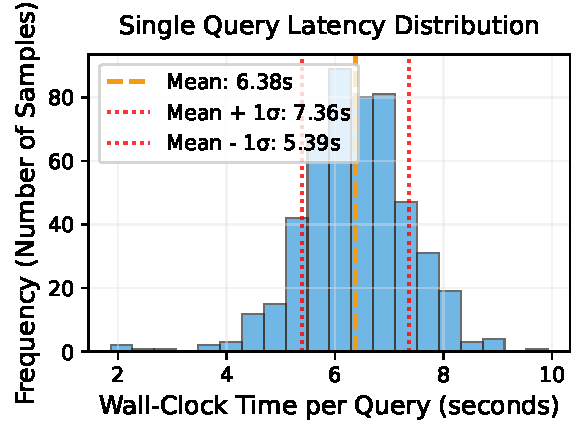
\includegraphics[width=\linewidth]{Figures/fig2_single_query_histogram.pdf}
    \caption{Histogram of end-to-end latency per question.}
    \label{fig:latency_hist}
  \end{subfigure}
  \begin{subfigure}{0.43\linewidth}
    \centering
    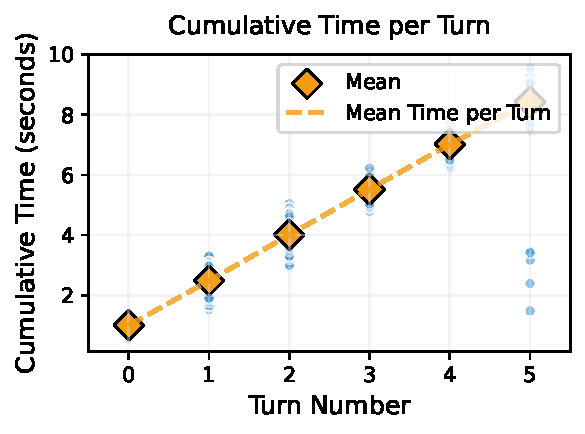
\includegraphics[width=\linewidth]{Figures/fig2_turn_time_scatter.pdf}
    \caption{Cumulative time by agent turn within a query.}
    \label{fig:turn_time_scatter}
  \end{subfigure}

  \caption{Single-query latency of \framework{} on an NVIDIA H100. 
  (a) Distribution of end-to-end latency; the dashed line marks the mean \(6.38\)\,s, and dotted lines indicate mean\(\ \pm\  1\sigma\) (\(5.39\)–\(7.36\) s). 
  (b) Cumulative time versus turn number across 500 queries; diamonds show per-turn means and the dashed trend denotes the average time per turn. The average maximum turn count is \(4.2\), and the near-linear growth indicates predictable per-turn costs suitable for interactive KGQA.}
  \label{fig:latency_histogram}
\end{figure}

\noindent \textbf{Batched Throughput}
We evaluate batched inference at batch size \(64\) on a single NVIDIA H100 (Table~\ref{tab:batched_throughput}). 
LLM-only baselines (no KG calls) achieve high throughput—\(81.8\) (IO) and \(70.1\) (CoT) samples/s—driven by short generation (43.0/206.0 tokens per sample).
\framework{} incurs KG-server retrieval, reducing throughput but remaining practical for offline processing: the single-run setting reaches \(3.7\) samples/s (\(1205.9\) gen tokens/s) with \(4.4\) KG calls per query, while the \(N{=}4\) runs setting trades throughput for more KG interaction (\(17.5\) calls per query), yielding \(2.0\) samples/s (\(612.1\) gen tokens/s).
Overall, \framework{} sustains batch processing on one H100 while supporting KG-grounded reasoning.

\begin{table}[ht]
\centering
\caption{Batched throughput on one NVIDIA H100 (256 queries; batch size 64).
\emph{Samples}: total queries. \emph{Batch}: batch size. \emph{KG Calls}: total KG-server requests.
\emph{Calls/Sample}: average KG requests per query. \emph{Total (s)}: end-to-end wall-clock time.
\emph{Gen Tok./Sample}: generated tokens per query. \emph{Samples/s}: queries per second.
\emph{Gen Tok./s}: generated tokens per second.}
\label{tab:batched_throughput}
\small
\setlength{\tabcolsep}{4pt}
\begin{adjustbox}{width=0.9\linewidth}
\begin{tabular}{@{}l|r|r|r|r|r|r|r|r@{}}
\toprule
\textbf{Configuration} & \textbf{Samples} & \textbf{Batch} & \textbf{KG Calls} & \textbf{Calls/Sample} & \textbf{Total (s)} & \textbf{Gen Tok./Sample} & \textbf{Samples/s} & \textbf{Gen Tok./s} \\
\midrule
IO              & 256 & 64 & 0    & 0.0  & 12.4  & 43.0  & 81.8 & 887.7 \\
CoT                   & 256 & 64 & 0    & 0.0  & 14.1  & 206.0 & 70.1 & 3740.1 \\
\framework{} (single run)   & 256 & 64 & 1127 & 4.4  & 73.2  & 345.0 & 3.7  & 1205.9 \\
\framework{} ($N{=}4$ runs) & 256 & 64 & 4478 & 17.5 & 142.2 & 340.0 & 2.0  & 612.1 \\
\bottomrule
\end{tabular}
\end{adjustbox}
\end{table}




\subsection{Ablation Studies}
\label{appendix:ablations}
All ablations in Table~\ref{tab:ablation_study_colored} evaluate \framework{} with Qwen-2.5-3B-it trained on \dataset{WebQSP} and \dataset{CWQ} using a maximum turn budget of \(H{=}5\).
We report the full ablation table in Table~\ref{tab:ablation_study_colored} and training curves in Figures~\ref{fig:ablation_training_curve_webqsp}.

\noindent \textbf{Turn Reward.} We vary the turn-level reward by setting the weights to \(w_{\text{fmt}}{=}0\), \(w_{\text{kg}}{=}0\), and \(w_{\text{ans}}{=}0\) (the default is \(0.5\) for all weights).

\noindent \textbf{Turn-level Advantage.} Instead of computing the turn-level group advantage \(A_t^{(n)}\) in Sec.~\ref{sub:kg_r1_rl}, we compute a trajectory-wise group advantage
\[
A_t^{(n)} \;=\; \frac{G^{(n)}-\bar{G}}{\sigma_{G}+\epsilon},\qquad
G^{(n)} \;=\; \frac{1}{T}\sum_{t} r_{t}^{\text{turn},(n)} \;+\; R^{\text{global},(n)},
\]
and use it for token-level credit assignment.

\noindent \textbf{Retrieval Reward.} We ablate the retrieval component by setting the weight \(w_{\text{ret}}{=}0\) (the default is \(1\)).

\noindent \textbf{RL Algorithm: GRPO vs.\ PPO.} We replace GRPO with vanilla PPO (VERL~\citep{sheng2024hybridflow} defaults), and set the turn-reward mixture weight \(w_{\text{turn}}{=}0\) (default: \(0.5\)). Advantage estimation is performed by a learned value critic (Qwen-2.5-3B-it).

\noindent \textbf{Hierarchical Relation Retrieval.} We change the KG-server retrieval format from a flat list to a hierarchical format that mirrors ``domain.type.property'' (see Table~\ref{tab:hierarchical_relation_format}).

\noindent \textbf{Base LLM Parameter Size (7B).} We swap the backbone from \textbf{Qwen-2.5-3B-it} to \textbf{Qwen-2.5-7B-it} while keeping data, rewards, and budgets fixed.

\subsubsection{Training curves}

\begin{figure}[H]
    \centering

    \begin{subfigure}{1.0\textwidth}
        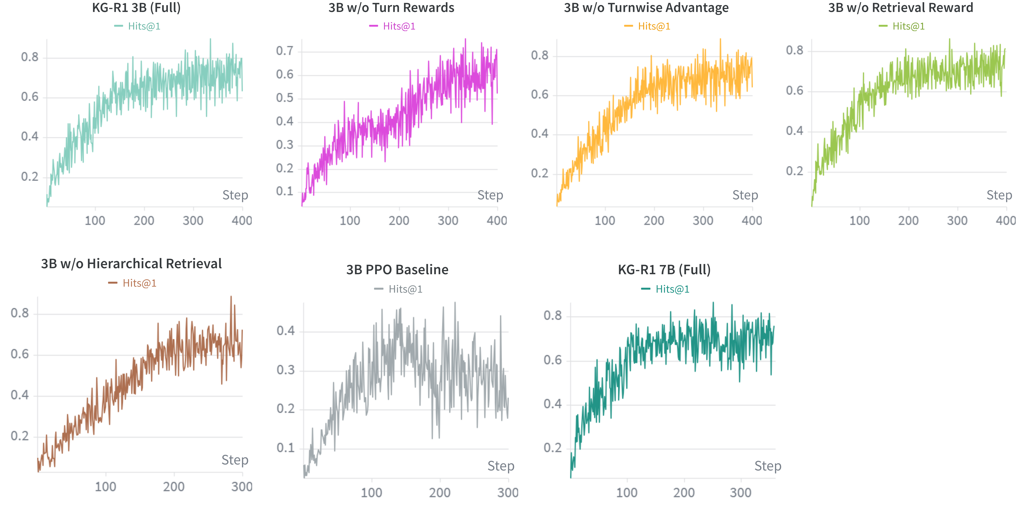
\includegraphics[width=\linewidth]{Figures/ablation_curve.png}
    \end{subfigure}

    \caption{Training curves of ablation studies, reporting Hits@1 across training steps.}
    \label{fig:ablation_training_curve_webqsp}
\end{figure}


\subsubsection{Hierachical Retrieval Format}
\label{appendix:hiearchical retreival}

Hierarchical retrieval format groups Freebase relations by their dot-notation structure (e.g., domain → type → property), presenting them as a compact tree instead of a flat comma-separated list. In the example (see Table~\ref{tab:hierarchical_relation_format}), this formatting preserves the same information while reducing verbosity—79 tokens vs.\ 156 tokens ($\approx$49\% fewer tokens).

\newcolumntype{L}[1]{>{\raggedright\arraybackslash\footnotesize}p{#1}}
\setlength{\tabcolsep}{5pt}
\renewcommand{\arraystretch}{1.05}


  
\begin{longtable}{|L{0.46\textwidth}|L{0.46\textwidth}|}
\caption{Hierarchical relation retrieval formatting used in KG\text{-}R1 to organize Freebase relations.}

\label{tab:hierarchical_relation_format}\\
\hline
\textbf{Flat Format} & \textbf{Hierarchical Format} \\
\hline
\endfirsthead
\hline
\textbf{Flat Format} & \textbf{Hierarchical Format} \\
\hline
\endhead
\small\sffamily
\textless kg-query\textgreater\par
get\_tail\_relations("m.09c7w0")\par
\textless /kg-query\textgreater\par
\vspace{4pt} %
\textless information\textgreater\ Tail relations for "m.09c7w0":\par
\vspace{4pt}%
location.country.first\_level\_divisions, location.location.containedby,
location.location.contains, people.person.nationality,
people.person.place\_of\_birth, government.government.government\_for\par
\textless /information\textgreater\par
\vspace{10pt}
\textbf{Result:} \textit{156 tokens}
&
\small\sffamily
\textless kg-query\textgreater\par
get\_tail\_relations("m.09c7w0")\par
\textless /kg-query\textgreater\par
\vspace{4pt}
\textless information\textgreater\ Tail relations for "m.09c7w0":\par
\vspace{4pt}%
location\par
\hspace*{2em}country: first\_level\_divisions\par
\hspace*{2em}location: containedby, contains\par
people\par
\hspace*{2em}person: nationality, place\_of\_birth\par
government\par
\hspace*{2em}government: government\_for\par
\textless /information\textgreater\par
\vspace{10pt}
\textbf{Result:} \textit{79 tokens (49.4\% savings)}\\
\hline
\end{longtable}



\subsubsection{PPO Reward Hacking }
The following \Cref{tab:fake_kg_information} shows the PPO reward hacking examples.
\label{appendix:reward_hacking_ppo}

\begin{longtable}{|L{0.46\textwidth}|L{0.46\textwidth}|}
  \caption{Policy model reward hacking under PPO. The actor model generates fake KG information that the
  critic model cannot distinguish from real data. \textcolor{blue}{Blue} denotes responses generated by the \framework{} agent.}
  \label{tab:fake_kg_information}\\
  \hline
  \textbf{Normal KG Retrieval} & \textbf{Fake Information Generated by Actor Policy in PPO} \\
  \hline
  \endfirsthead
  \hline
  \textbf{Real KG Retrieval} & \textbf{Fake Information Generated by Policy} \\
  \hline
  \endhead

  \small\sffamily
  \textbf{Question:} Who directed the movie Inception?\par
  \vspace{4pt}
  \begin{blueblock}
  {\lt}kg-query{\gt}\par
  get\_head\_entities("film.film.directed\_by", "Inception")\par
  {\lt}/kg-query{\gt}\par
  \end{blueblock}
  \vspace{4pt}
  {\lt}information{\gt} Head entities for relation
  ``film.film.directed\_by'' with tail ``Inception'':\par
  \vspace{2pt}%
  Christopher Nolan (m.04f9z)\par
  {\lt}/information{\gt}\par
  \vspace{6pt}
  \textbf{Answer:} Christopher Nolan directed Inception.
  &
  \small\sffamily
  \textbf{Question:} Who directed the movie Inception?\par
  \vspace{4pt}
  \begin{blueblock}
  {\lt}kg-query{\gt}\par
  get\_head\_entities("film.film.directed\_by", "Inception")\par
  {\lt}/kg-query{\gt}\par
  \end{blueblock}
  \vspace{4pt}
  {\lt}information{\gt} Head entities for relation
  ``film.film.directed\_by'' with tail ``Inception'':\par
  \vspace{2pt}%
  Christopher Nolan, Barack Obama, Elon Musk, Albert Einstein, Michael Jordan\par
  {\lt}/information{\gt}\par
  \vspace{6pt}
  \textbf{Answer:} Inception was directed by Christopher Nolan, with creative input from Barack Obama, Elon Musk,
  Albert Einstein, and Michael Jordan as co-directors.\\
  \hline
\end{longtable}








\newpage
\section{Examples of Responses}

\label{Appendix:responses}
\begin{table}[H]
\centering
\caption{Example \framework{} response on \dataset{WebQSP}, showing multi-step reasoning and verification for a person-children query. \textcolor{blue}{Blue} denotes responses generated by the \framework{} agent.}
\begin{reasonbox}[title=\framework{} Response Example — \dataset{WebQSP}]
Question: What are Victoria Beckham's kids' names?
Initial entities : 'Victoria Beckham'
\vspace{0.5em}\hrule\vspace{0.5em}

\begin{blueblock}
\texttt{<think>}\\
I need to find out the names of Victoria Beckham's kids. I will start by finding any relations to her children.\\
\texttt{</think>}\\
\texttt{<kg-query>}\\
$\gettailrelations(\text{"Victoria Beckham"})$\\
\texttt{</kg-query>}
\end{blueblock}

\vspace{0.5em}\hrule\vspace{0.5em}

\texttt{<information>} Tail relations for entity "Victoria Beckham":\\
base.popstra.celebrity.breakup, award.award\_nominee.award\_nominations, \dots, people.person.children, \dots
\texttt{</information>}

\vspace{0.5em}\hrule\vspace{0.5em}

\begin{blueblock}
\texttt{<think>}\\
The relation \texttt{people.person.children} is relevant. I will use it to get the names of her children.\\
\texttt{</think>}\\
\texttt{<kg-query>}\\
$\gettailentities(\text{"Victoria Beckham"}, \text{"people.person.children"})$\\
\texttt{</kg-query>}
\end{blueblock}

\vspace{0.5em}\hrule\vspace{0.5em}

\texttt{<information>} Tail entities for relation "people.person.children":\\
Brooklyn Joseph Beckham, Cruz David Beckham, Harper Seven Beckham, Romeo James Beckham
\texttt{</information>}

\vspace{0.5em}\hrule\vspace{0.5em}

\begin{blueblock}
\texttt{<think>}\\
The names of Victoria Beckham's children are found. I will verify by checking each child's parent relation.\\
\texttt{</think>}\\
\texttt{<kg-query>}\\
$\getheadrelations(\text{"Brooklyn Joseph Beckham"})$\\
\texttt{</kg-query>}
\end{blueblock}

\vspace{0.5em}\hrule\vspace{0.5em}

\texttt{<information>} Head relations for "Brooklyn Joseph Beckham":\\
base.godparents.godparent.godchildren, people.person.children, people.sibling\_relationship.sibling
\texttt{</information>}

\vspace{0.5em}\hrule\vspace{0.5em}

\begin{blueblock}
\texttt{<think>}\\
Confirming Brooklyn's parents using \texttt{people.person.children}.\\
\texttt{</think>}\\
\texttt{<kg-query>}\\
$\getheadentities(\text{"Brooklyn Joseph Beckham"}, \text{"people.person.children"})$\\
\texttt{</kg-query>}
\end{blueblock}

\vspace{0.5em}\hrule\vspace{0.5em}

\texttt{<information>} Head entities for relation with tail "Brooklyn Joseph Beckham":\\
David Beckham, Victoria Beckham
\texttt{</information>}

\vspace{0.5em}\hrule\vspace{0.5em}

\texttt{<think>} Brooklyn, Cruz, Harper, and Romeo all confirm to have David and Victoria Beckham as parents. \texttt{</think>}

\begin{blueblock}
\texttt{<answer>}\\
Brooklyn Joseph Beckham, Cruz David Beckham, Harper Seven Beckham, Romeo James Beckham\\
\texttt{</answer>}
\end{blueblock}

\vspace{0.5em}\hrule\vspace{0.5em}
\vspace{0.1em}\hrule\vspace{0.5em}
\textbf{[ground\_truth]} \{‘Brooklyn Joseph Beckham’, ‘Romeo James Beckham’, ‘Cruz David Beckham’, ‘Harper Seven Beckham’\}
\end{reasonbox}
\end{table}





\begin{table}[H]
\centering
\caption{Example \framework{} response in \dataset{CWQ}. \textcolor{blue}{Blue} denotes responses generated by the \framework{} agent.}
\begin{reasonbox}[title=\framework{} Response Example - \dataset{CWQ}]
Question: What movie, written by Mike Jefferies, starred Nick Cannon? \\
Initial entities: "Mike Jefferies", "Nick Cannon"
\vspace{0.5em}\hrule\vspace{0.5em}
\begin{blueblock}
\texttt{<think>} \\
Let's start by finding a movie written by Mike Jefferies. We can use the relation that associates writers with their movies. \\
\texttt{</think>} \\
\texttt{<kg-query>} \\
$\gettailrelations$(\text{"Mike Jefferies"})
\texttt{</kg-query>} 
\end{blueblock}
\vspace{0.5em}\hrule\vspace{0.5em}
\texttt{<information>}Tail relations for entity "Mike Jefferies": \\
film.film\_story\_contributor.film\_story\_credits, people.person.nationality, people.person.place\_of\_birth, film.writer.film,  ... \texttt{</information>}
\vspace{0.5em}\hrule\vspace{0.5em}
\begin{blueblock}
\texttt{<think>} \\
From the initial query results, we have two possible options for Mike Jefferies' work. Let's start with "film.writer.film" to find the movies written by Mike Jefferies and then see if Nick Cannon starred in any of those films. \\
\texttt{</think>} \\
\texttt{<kg-query>} \\
$\gettailentities$("Mike Jefferies", "film.writer.film") \\
\texttt{</kg-query>}
\end{blueblock}
\vspace{0.5em}\hrule\vspace{0.5em}
\texttt{<information>}Tail entities for relation "film.writer.film" with head "Mike Jefferies": Goal II: Living the Dream, Goal III: Taking on the World\texttt{</information>} 
\vspace{0.5em}\hrule\vspace{0.5em}
\begin{blueblock}
\texttt{<think>} \\
Now that we have two movies written by Mike Jefferies, let's check if Nick Cannon has starred in any of these movies. We'll use the relation that connects actors with the movies they star in. \\
\texttt{</think>}
\texttt{<kg-query>} \\
$\getheadrelations$("Nick Cannon") \\
\texttt{</kg-query>} 
\end{blueblock}
\vspace{0.5em}\hrule\vspace{0.5em}
\texttt{<information>}Head relations for entity "Nick Cannon": 
base.popstra.dated.participant, film.personal\_film\_appearance.person, music.album.primary\_release, \\base.popstra.lived\_with.participant, film.film.written\_by, ... \texttt{</information>}
\vspace{0.5em}\hrule\vspace{0.5em}
...
\\
...
\\
...
\vspace{0.5em}\hrule\vspace{0.5em}
\begin{blueblock}
\texttt{<think>} \\
From the relations where "Goal II: Living the Dream" is involved, we can see that it is a film with a writer, which aligns with Mike Jefferies. \\
\texttt{</think>} \\
\texttt{<answer>} \\
Goal II: Living the Dream, School Dance, School Gyrls, Goal III: Taking on the World \\
\texttt{</answer>}
\end{blueblock}
\vspace{0.5em}\hrule\vspace{0.5em}
\vspace{0.1em}\hrule\vspace{0.5em}

\textbf{[ground\_truth]} \{'Goal II: Living the Dream' \}
\end{reasonbox}
\end{table}

\begin{table}[H]
\centering
\caption{Example \framework{} response in \dataset{SimpleQA}. \textcolor{blue}{Blue} denotes responses generated by the \framework{} agent.}
\begin{reasonbox}[title=\framework{} Response Example - \dataset{SimpleQA}]
Question: Where is the madam satan located? (Initial entities: "Madam Satan") \\
\vspace{0.5em}\hrule\vspace{0.5em}
\begin{blueblock}
\texttt{<think>} \\
I need to find out where Madam Satan is located. First, I will check if it has a location or if it's an entity that can be queried about its location. \\
\texttt{</think>} \\
\texttt{<kg-query>} \\
$\gettailrelations(\text{"Madam Satan"})$ \\
\texttt{</kg-query>}
\end{blueblock}

\vspace{0.5em}\hrule\vspace{0.5em}

\texttt{<information>}Tail relations for entity "Madam Satan": \\
film.film.cinematography, common.topic.notable\_types, film.film.language, 
film.film.starring,film.film.country,   ... award.ranked\_item.appears\_in\_ranked\_lists,  
film.film.film\_art\_direction\_by\texttt{</information>}

\vspace{0.5em}\hrule\vspace{0.5em}

\begin{blueblock}
\texttt{<think>} \\
None of the identified relations are directly related to location. Let me check if Madam Satan is detailed in a geographical context. \\
\texttt{</think>} \\
\texttt{<kg-query>} \\
$\gettailentities(\text{"Madam Satan"}, \text{"film.film.country"})$ \\
\texttt{</kg-query>}
\end{blueblock}

\vspace{0.5em}\hrule\vspace{0.5em}

\texttt{<information>}Tail entities for relation "film.film.country" with head "Madam Satan": United States of America\texttt{</information>}

\vspace{0.5em}\hrule\vspace{0.5em}

\begin{blueblock}
\texttt{<think>} \\
I have found that Madam Satan, identified as a film, is located in the United States of America. However, it's crucial to confirm the specific location or city within the country where Madam Satan was filmed. \\
\texttt{</think>} \\
\texttt{<kg-query>} \\
$\gettailentities(\text{"Madam Satan"}, \text{"film.film.starring"})$ \\
\texttt{</kg-query>}
\end{blueblock}

\vspace{0.5em}\hrule\vspace{0.5em}
..\\
..\\
..
\vspace{0.5em}\hrule\vspace{0.5em}

\texttt{<information>}Tail entities for relation "film.film.runtime" with head "Madam Satan": m.03kx9f2\texttt{</information>}

\vspace{0.5em}\hrule\vspace{0.5em}

\begin{blueblock}
\texttt{<think>} \\
I am still not obtaining the most helpful information about the location. Possibly Madam Satan was released, but not filmed in a specific place. \\
\texttt{</think>} \\
\texttt{<kg-query>} \\
$\getheadrelations(\text{"m.02tb01n"})$ \\
\texttt{</kg-query>}
\end{blueblock}

\vspace{0.5em}\hrule\vspace{0.5em}

\texttt{<information>}Head relations for entity "m.02tb01n": \\
film.film.starring, film.actor.film\texttt{</information>}

\vspace{0.5em}\hrule\vspace{0.5em}

\begin{blueblock}
\texttt{<think>} \\
I have questioned the relation "film.actor.film". This relation includes the movies the actor is in. Let's try to find a clearer detail for the location of Madam Satan. \\
\texttt{</think>} \\
\texttt{<answer>} \\
United States of America \\
\texttt{</answer>}
\end{blueblock}
\vspace{0.5em}\hrule\vspace{0.5em}
\vspace{0.1em}\hrule\vspace{0.5em}

\textbf{[ground\_truth]} \{'United States of America' \}


\end{reasonbox}
\end{table}


\begin{table}[H]
\centering
\caption{Example \framework{} response in \dataset{T-REx}. \textcolor{blue}{Blue} denotes responses generated by the \framework{} agent.}
\begin{reasonbox}[title=\framework{} Response Example — \dataset{T-REx}]
Question: What is the instance of Solberg?? \\
Initial entities: "Solberg"
\vspace{0.5em}\hrule\vspace{0.5em}

\begin{blueblock}
\texttt{<think>} \\
Let's start with the entity Solberg and try to find out what it represents. It seems like Solberg could be an entity that describes a geopolitical boundary, location, or characterization. The query can be adjusted from general to specific as needed. \\
\texttt{</think>} \\
\texttt{<kg-query>} \\
$\gettailrelations(\text{"Solberg"})$ \\
\texttt{</kg-query>}
\end{blueblock}

\vspace{0.5em}\hrule\vspace{0.5em}
\texttt{<information>}Tail relations for entity "Solberg": P1889, P407, P1552, P282, P31, P460\texttt{</information>}
\vspace{0.5em}\hrule\vspace{0.5em}

\begin{blueblock}
\texttt{<think>} \\
The relations provided show how Solberg is related to other entities. Let's explore each relation to find out more about Solberg. \\
\texttt{</think>} \\
\texttt{<kg-query>} \\
$\gettailentities(\text{"Solberg"},\ \text{"P282"})$ \\
\texttt{</kg-query>}
\end{blueblock}

\vspace{0.5em}\hrule\vspace{0.5em}

\texttt{<information>}Tail entities for relation "P282" with head "Solberg": Latin script\texttt{</information>}

\vspace{0.5em}\hrule\vspace{0.5em}

\begin{blueblock}
\texttt{<think>} \\
The relation P282 corresponds to "type.object.name" according to the API documentation, indicating that Solberg is a human name. The relation P407 is also noteworthy but does not give further specific information. Let's try a broader query for more context related to Solberg. \\
\texttt{</think>} \\
\texttt{<kg-query>} \\
$\gettailentities(\text{"Solberg"},\ \text{"P31"})$ \\
\texttt{</kg-query>}
\end{blueblock}
\vspace{0.5em}\hrule\vspace{0.5em}
\texttt{<information>}Tail entities for relation "P31" with head "Solberg": Wikimedia disambiguation page, family name\texttt{</information>}
\vspace{0.5em}\hrule\vspace{0.5em}
...\\
...\\
...
\vspace{0.5em}\hrule\vspace{0.5em}

\begin{blueblock}
\texttt{<think>} \\
The retrieval of "Soelberg", "Sohlberg", and "Sohlberg" suggests that Solberg might be associated with these names. To find an instance of Solberg, we can search for a specific entity of this name. \\
\texttt{</think>} \\
\texttt{<answer>} \\
Latin script, Wikimedia disambiguation page, family name, Soelberg, Sohlberg, Sohlberg \\
\texttt{</answer>}

\end{blueblock}
\vspace{0.5em}\hrule\vspace{0.5em}
\vspace{0.1em}\hrule\vspace{0.5em}

\textbf{[ground\_truth]} \{'family name', 'human settlement', 'urban area in Sweden', 'minor locality in Sweden', 'minor locality in Sweden', 'Wikimedia disambiguation page', 'human settlement', 'Ortsteil', 'stone setting', 'human settlement', 'minor locality in Sweden', 'hill', 'stone setting', 'hill', 'human settlement' \}

\end{reasonbox}
\end{table}

\begin{table}[H]
\centering
\caption{Example \framework{} response in \dataset{QALD10en}. \textcolor{blue}{Blue} denotes responses generated by the \framework{} agent.}
\begin{reasonbox}[title=\framework{} Response Example - \dataset{QALD10en}]
Question: After whom is the Riemannian geometry named?? (Initial entities: "Riemannian geometry") \\
\vspace{0.5em}\hrule\vspace{0.5em}

\begin{blueblock}
\texttt{<think>} \\
I need to find out who the Riemannian geometry is named after. Let's start by investigating the relations and entities connected to "Riemannian geometry". \\
\texttt{</think>} \\
\texttt{<kg-query>} \\
$\gettailrelations(\text{"Riemannian geometry"})$ \\
\texttt{</kg-query>}
\end{blueblock}

\vspace{0.5em}\hrule\vspace{0.5em}

\texttt{<information>}Tail relations for entity "Riemannian geometry": \\
on focus list of Wikimedia project, named after, maintained by WikiProject, topic's main category, instance of, subclass of\texttt{</information>}

\vspace{0.5em}\hrule\vspace{0.5em}

\begin{blueblock}
\texttt{<think>} \\
From the relations extracted, it appears the Riemannian geometry is named after someone. I will now search for the person it's named after. \\
\texttt{</think>} \\
\texttt{<kg-query>} \\
$\gettailentities(\text{"Riemannian geometry"}, \text{"named after"})$ \\
\texttt{</kg-query>}
\end{blueblock}

\vspace{0.5em}\hrule\vspace{0.5em}

\texttt{<information>}Tail entities for relation "named after" with head "Riemannian geometry": Bernhard Riemann\texttt{</information>}

\vspace{0.5em}\hrule\vspace{0.5em}

\begin{blueblock}
\texttt{<think>} \\
I now have the information that the Riemannian geometry is named after Bernhard Riemann. Let's confirm this by checking if there's more detailed information about this relationship. \\
\texttt{</think>} \\
\texttt{<kg-query>} \\
$\getheadrelations(\text{"Bernhard Riemann"})$ \\
\texttt{</kg-query>}
\end{blueblock}

\vspace{0.5em}\hrule\vspace{0.5em}

\texttt{<information>}Head relations for entity "Bernhard Riemann": \\
named after\texttt{</information>}

\vspace{0.5em}\hrule\vspace{0.5em}

\begin{blueblock}
\texttt{<think>} \\
These results are confirming that Bernhard Riemann is indeed the person the Riemannian geometry is named after. No further information is needed. \\
\texttt{</think>} \\
\texttt{<kg-query>} \\
$\getheadentities(\text{"Bernhard Riemann"}, \text{"named after"})$ \\
\texttt{</kg-query>}
\end{blueblock}

\vspace{0.5em}\hrule\vspace{0.5em}

\texttt{<information>}Head entities for relation "named after" with tail "Bernhard Riemann": Riemannian geometry\texttt{</information>}

\vspace{0.5em}\hrule\vspace{0.5em}

\begin{blueblock}
\texttt{<think>} \\
This confirms my findings; the Riemannian geometry is named after Bernhard Riemann. \\
\texttt{</think>} \\
\texttt{<answer>} \\
Bernhard Riemann \\
\texttt{</answer>}
\end{blueblock}

\vspace{0.5em}\hrule\vspace{0.5em}
\vspace{0.1em}\hrule\vspace{0.5em}

\textbf{[ground\_truth]} \{'Bernhard Riemann'\}

\end{reasonbox}
\end{table}



\begin{table}[H]
\centering
\caption{Example \framework{} response in \dataset{GrailQA}. \textcolor{blue}{Blue} denotes responses generated by the \framework{} agent.}
\begin{reasonbox}[title=\framework{} Response Example — \dataset{GrailQA}]
Question: What video game is published by softdisk? \\
Initial entities: "Near West Side"
\vspace{0.5em}\hrule\vspace{0.5em}

\begin{blueblock}
\texttt{<think>} \\
First, I need to find out what game is published by Softdisk. Without specific knowledge about "Near West Side", I will start with the game publisher for Softdisk. \\
\texttt{</think>} \\
\texttt{<kg-query>} \\
$\getheadrelations(\text{"Near West Side"})$ \\
\texttt{</kg-query>}
\end{blueblock}

\vspace{0.5em}\hrule\vspace{0.5em}

\texttt{<information>}Head relations for entity "Near West Side": \\
book.periodical\_publisher\_period.publisher, business.industry.companies, business.employment\_tenure.company\texttt{</information>}

\vspace{0.5em}\hrule\vspace{0.5em}

\begin{blueblock}
\texttt{<think>} \\
The head relation "business.employment\_tenure.company" suggests that "Near West Side" might be a game company or related to a game. I will try to find out the publisher of a game related to "Near West Side" by looking for games published by Softdisk. \\
\texttt{</think>} \\
\texttt{<kg-query>} \\
$\gettailrelations(\text{"Near West Side"})$ \\
\texttt{</kg-query>}
\end{blueblock}

\vspace{0.5em}\hrule\vspace{0.5em}

\texttt{<information>}Tail relations for entity "Near West Side": \\
organization.organization.place\_founded, organization.organization.headquarters, book.periodical\_publisher.periodicals\_published, business.employer.employees, cvg.cvg\_publisher.games\_published, business.business\_operation.industry, common.topic.notable\_types\texttt{</information>}

\vspace{0.5em}\hrule\vspace{0.5em}
...\\
...\\
...\\
\vspace{0.5em}\hrule\vspace{0.5em}

\begin{blueblock}
\texttt{<think>} \\
The previous query did not provide a conclusive answer. Let's try a different approach by checking if "Augusto Cury" is associated with any game publishers. \\
\texttt{</think>} \\
\texttt{<answer>} \\
Augusto Cury, Catacomb 3-D, Chagunitzu, Dangerous Dave in the Haunted Mansion, Hovertank 3D, Iron Seed, Lado Skorin, North Cambridge Academy, Roberto Torretti, Shadow Knights, Star Film Company, Tiles of the Dragon \\
\texttt{</answer>}
\end{blueblock}


\vspace{0.5em}\hrule\vspace{0.5em}
\vspace{0.1em}\hrule\vspace{0.5em}

\textbf{[ground\_truth]} \{'Rescue Rover','Catacomb 3-D','Shadow Knights',"Dangerous Dave's Risky Rescue",'Tiles of the Dragon', 'Catacomb', 'Commander Keen: Keen Dreams', 'Dave Goes Nutz!','Chagunitzu','Dangerous Dave in the Haunted Mansion','Hovertank 3D','Iron Seed'\}


\end{reasonbox}
\end{table}






























